\documentclass[]{article}
\usepackage{amsmath}
\usepackage{amssymb}
\usepackage{subcaption}
\usepackage{graphicx}
\usepackage{float}
\usepackage{multicol}


%\usepackage{easyReview} %used for annotation. Cannot be run together with (changes) - command "highlight" defined twice
\usepackage{changes}%use while actively annotating

%\usepackage[final]{changes} % once we are happy with all annotation, we can accept all proposed changes and show only the final document.

% simply select text you want to annotate and start typing the command \replacedGM{the selected text will appear here}{and here you enter the new replacement text}
\definechangesauthor[name={Timo}, color=orange]{tp}
\definechangesauthor[name={Giovanni}, color=green]{gm}
\newcommand{\replacedTP}[2]{\replaced[id=tp]{#2}{#1}}
\newcommand{\addedTP}[1]{\added[id=tp]{#1}}
\newcommand{\deletedTP}[1]{\deleted[id=tp]{#1}}
\newcommand{\highlightTP}[1]{\highlight[id=tp]{#1}}
\newcommand{\commentTP}[2]{\comment[id=tp]{#2}{#1}}

\newcommand{\replacedGM}[2]{\replaced[id=gm]{#2}{#1}}
\newcommand{\addedGM}[1]{\added[id=gm]{#1}}
\newcommand{\deletedGM}[1]{\deleted[id=gm]{#1}}
\newcommand{\highlightGM}[1]{\highlight[id=gm]{#1}}
\newcommand{\commentGM}[2]{\comment[id=gm]{#2}{#1}}

%opening
\title{}
\author{}

\begin{document}
	
	\maketitle
	
	
	\section*{Question 4: Testing the CAPM}
	\subsection*{a. replication of Cochrane's graph 15.1 and 15.2}
	
	The referred figures are:
	
	\begin{figure}
	\centering
	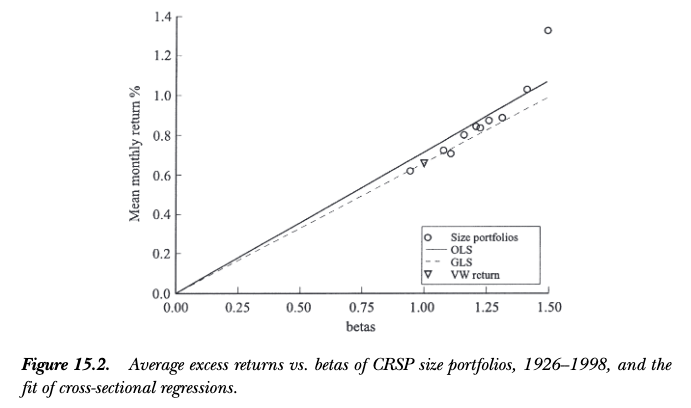
\includegraphics[width=0.7\linewidth]{Cochrane_15_2}
	\caption{}
	\label{fig:cochrane151}
\end{figure}
	
	
	\begin{figure}
		\centering
		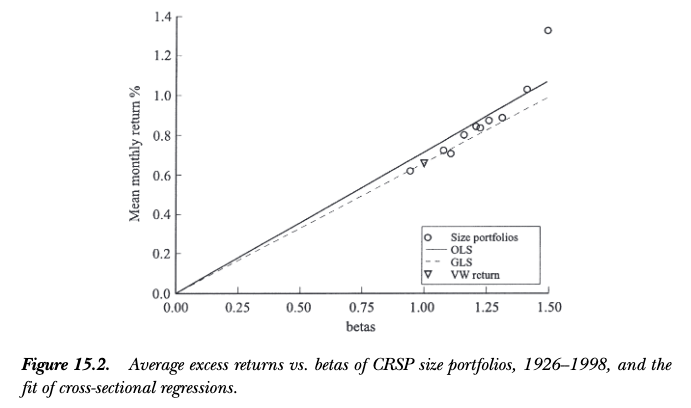
\includegraphics[width=0.7\linewidth]{Cochrane_15_2}
		\caption{}
		\label{fig:cochrane152}
	\end{figure}
	
	
	
\end{document}